\section{Vergelijkingsoverzicht}
\label{sec:evaluatie-spinnenweb}

% eerst de grafiek van onze initiële criteria en formules

\begin{figure}[H]
  \centering
  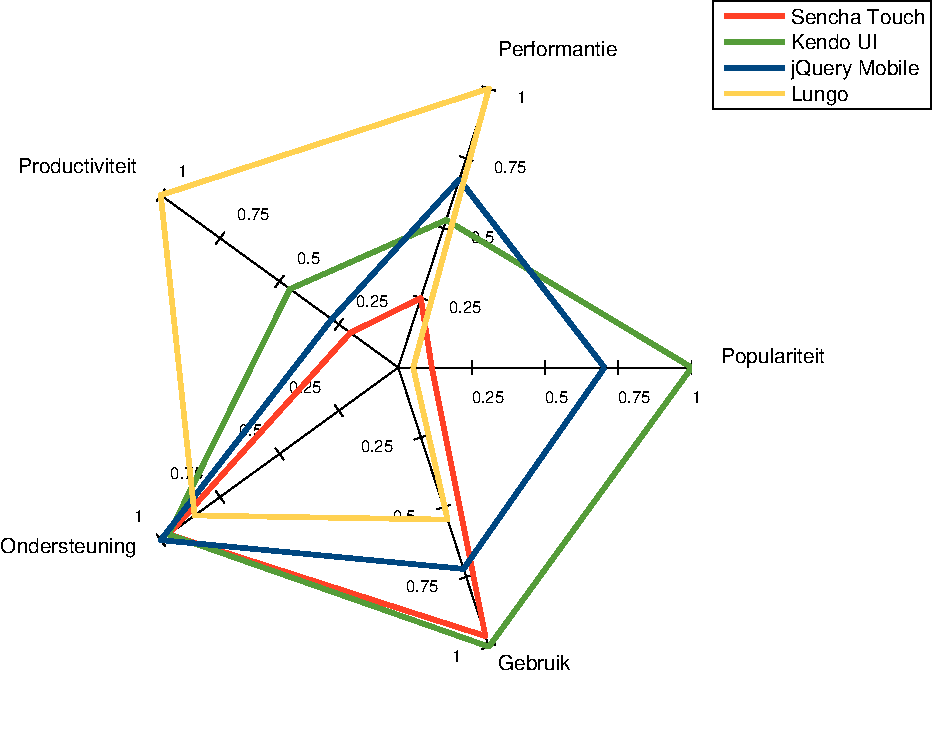
\includegraphics[width=\textwidth]{figuren/spidergraph-initial.pdf}
  \caption{Vergelijkingsoverzicht met de vijf vergelijkingscriteria voor \st{},  \kendo{},  \jqm{} en \lungo{}.}
  \label{fig:spinnenweb-initial}
\end{figure}

% besluiten  (de getallen zijn geen procenten)
% 1) Kendo: 1,51 
% 2) Lungo: 1,14
% 3) jQM: 1,03
% 4) ST: 0,62
% but...

% daarna de bindparagraaf door onze 2 improvents (productiviteit en performantie)
% referen naar de nieuwe formules in de respectievelijke secties
% nieuwe formules voor het bereken van het relatieve waarden voor de respectievelijke formules
% tonen van de finale grafiek

\begin{figure}[H]
  \centering
  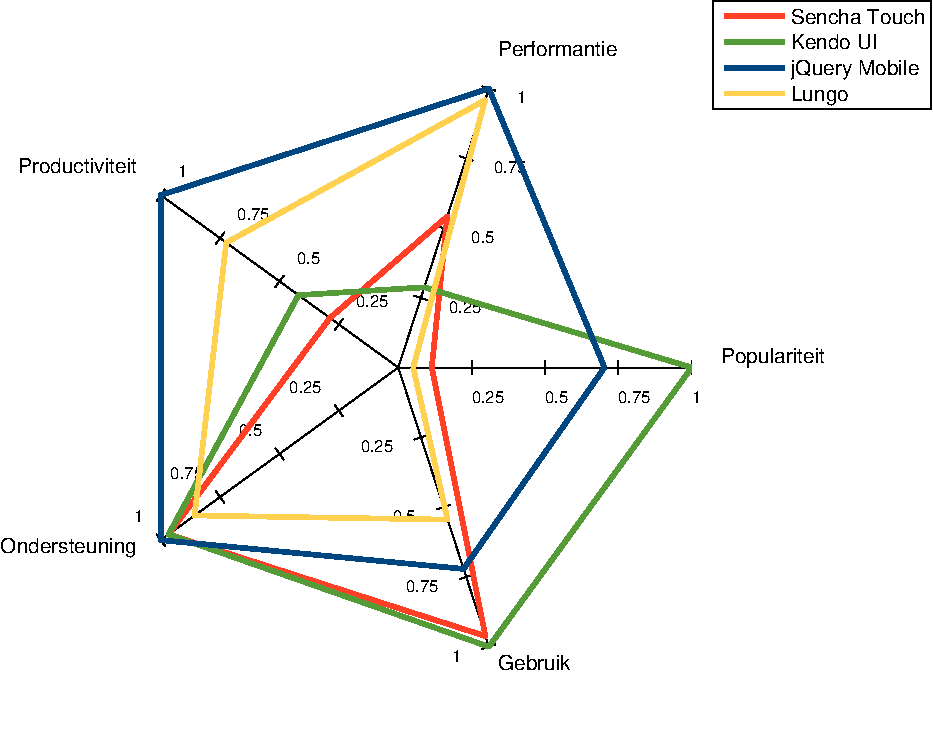
\includegraphics[width=\textwidth]{figuren/spidergraph-final.pdf}
  \caption{Vergelijkingsoverzicht met de vijf vergelijkingscriteria voor \st{},  \kendo{},  \jqm{} en \lungo{}.}
  \label{fig:spinnenweb-final}
\end{figure}

% Finale volgordes (de getallen zijn geen procenten)
% 1) jQM: 1,87
% 2) Kendo: 1,32
% 3) Lungo: 0,88
% 4) ST: 0,73
% but...